%# -*- coding: utf-8 -*-
%!TEX encoding = UTF-8 Unicode
%%%%%%%%%%%%%%%%%%%%%%%%%%%%%%%%%%%%%%%%%%%%%%%%%%%%%%%%%%%%%%%%%%%%%%%%%%%%%%%%%%
%论文模板                                                                        %
%此为中文XeLatex-article                                                         %
%                             !编译方式是:XeLaTeX  !                          %
%%%%%%%%%%%%%%%%%%%%%%%%%%%%%%%%%%%%%%%%%%%%%%%%%%%%%%%%%%%%%%%%%%%%%%%%%%%%%%%%%%
\documentclass[12pt]{article}
\usepackage[slantfont,boldfont]{xeCJK}% 允许斜体和粗体
\setCJKmainfont{FangSong}             % 设置缺省中文字体
\setmainfont{Times New Roman}         % 设置Times New Roman为默认的英文字体
\setlength{\parindent}{2.5em}         % 中文缩进两个汉字位

\usepackage{CJK}
\usepackage{cmap}  %解决复制乱码问题
\usepackage{titlesec}%章节标题格式设置
\usepackage{titletoc}%目录格式设置
\usepackage{amsmath}%公式环境数学命令
\usepackage{array}%数组和表格制作
\usepackage[a4paper,top=2.5cm,bottom=2.5cm,left=3cm,right=2cm]{geometry}% 版面尺寸设置
\usepackage{multirow}
\usepackage{enumerate}
\usepackage{verbatim,listings}
\usepackage{color,xcolor}
%\usepackage{graphicx}
\usepackage{slashbox}
\usepackage{fancybox}
\usepackage{fancyhdr}
\usepackage{float}    % for fig.pos='H'
\usepackage{rotfloat} % for sidewaysfigure
\usepackage{subfig}   % for subfigure
\usepackage{booktabs}

%%%%%%%%%%%%%%%%%%%%%%%%%%%%%%%%%%%%%%%%%%%%%%%%%%%%%%%%%%%%%%%%%%%%%%%%%%%%%%%%%%%%%%%%%%%%%%%%%%%%%
%自定义命令:
\makeatletter
%字号设置
\newcommand{\chuhao}{\fontsize{42pt}{\baselineskip}\selectfont}% 初号
\newcommand{\xiaochuhao}{\fontsize{36pt}{\baselineskip}\selectfont}% 小初号
\newcommand{\yihao}{\fontsize{28pt}{\baselineskip}\selectfont}% 一号
\newcommand{\erhao}{\fontsize{21pt}{\baselineskip}\selectfont}% 二号
\newcommand{\xiaoerhao}{\fontsize{18pt}{\baselineskip}\selectfont}% 小二号
\newcommand{\sanhao}{\fontsize{15.75pt}{\baselineskip}\selectfont}% 三号
\newcommand{\xiaosanhao}{\fontsize{15pt}{\baselineskip}\selectfont}% 小三号
\newcommand{\sihao}{\fontsize{14pt}{\baselineskip}\selectfont}% 四号
\newcommand{\xiaosihao}{\fontsize{12pt}{\baselineskip}\selectfont}% 小四号
\newcommand{\wuhao}{\fontsize{10.5pt}{\baselineskip}\selectfont}% 五号
\newcommand{\xiaowuhao}{\fontsize{9pt}{\baselineskip}\selectfont}% 小五号
\newcommand{\liuhao}{\fontsize{7.875pt}{\baselineskip}\selectfont}% 六号
\newcommand{\qihao}{\fontsize{5.25pt}{\baselineskip}\selectfont}% 七号

%行间距设置
\renewcommand\baselinestretch{1.25}%1.25倍行距

%页眉页脚设置1
\fancypagestyle{plain}
{
\fancyhead{}
\fancyhead[C]{\wuhao{数理与土木工程学院大数据系课程论文}}
\fancyfoot{}
\fancyfoot[C]{\thepage}
}
%页眉页脚设置2
\pagestyle{fancy}
{
 \fancyhead{}
 \fancyhead[C]{\wuhao{数理与土木工程学院大数据系课程论文}}
 \fancyfoot{}
}

%重新定义
\renewcommand\refname{参考文献}
\renewcommand\figurename{图}
\renewcommand\tablename{表}


%表格设置
\newsavebox{\tablebox}


\makeatother
%%%%%%%%%%%%%%%%%%%%%%%%%%%%%%%%%%%%%%%%%%%%%%%%%%%%%%%%%%%%%%%%%%%%%%%%%%%%%%%%%%%%%%%%%%%%%%%%%%%%%


\begin{document}

\lstset{numbers=left,
numberstyle= \tiny,
keywordstyle= \color{ blue!70},commentstyle=\color{red!50!green!50!blue!50},
frame=shadowbox,
rulesepcolor= \color{ red!20!green!20!blue!20}
}
\lstset{
  breaklines,%自动换行
  columns=flexible,%不随便添加空格,只在已经有空格的地方添加空格,
%如果想要添加空格使用fixed作为参数(这是默认的),如果坚决不添加空格使用fullflexible作为参数.
}

%%%%%%%%%%%%%%%%%%%%%%%%%%%%%%%%%%%%%%%%%%%%%%%%%%%%%%%%%%%%%%%%%%%%%%%%%%%%%%%%%%%%%%%%%%%%%%%%%%%%%%

%%%%%%%%%%%%%%%%%%封面%%%%%%%%%%%%%%%%%%%%%%%%%%%%%%%%%%%%%%%%%%%%%%%%%%%%%%%%%%%%%%%%%%%%%%%%%%%%%%%%%
\thispagestyle{empty}

\begin{center}

\includegraphics[height=0.15\textwidth]{figures/logo.jpg}

\vspace{4cm}

{\yihao\bf{关于医疗数据的数据可视化}}
\end{center}

\vspace{4cm}

{\xiaosanhao\bf
\begin{center}
\makebox[3cm][l]{学~~~~~~~~~院:}\underbar{\makebox[11cm][c]{数理与土木工程学院}}
\end{center}
\begin{center}
\makebox[3cm][l]{课~~~~~~~~~程:}\underbar{\makebox[11cm][c]{数据可视化}}
\end{center}
\begin{center}
\makebox[3cm][l]{班~~~~~~~~~级:}\underbar{\makebox[11cm][c]{数据科学与大数据技术1班}}
\end{center}
\begin{center}
\makebox[3cm][l]{姓~~~~~~~~~名:}\underbar{\makebox[4cm][c]{覃诗杰}}\makebox[3cm][l]{学~~~~~~~~~号:}\underbar{\makebox[4cm][c]{201205102261}}
\end{center}
}


\vspace{4cm}


\begin{center}\wuhao\bf
{
\makebox[5cm][c]{中国~$\cdot$~珠海}

\renewcommand{\today}{\number\year 年 \number\month 月 \number\day 日}
\today\\
%\makebox[5cm][c]{二〇二〇年六月}
}

\end{center}

%%%%%%%%%%%%%%%%%%%%%%%%以下命令生成中文摘要%%%%%%%%%%%%%%%%%%%%%%%%%%%%%%%%%%%%%%%%
\newpage
\thispagestyle{fancy}

\begin{center}
{\sanhao\textbf{医疗数据可视化}}
\end{center}

\renewcommand\abstractname{\xiaosanhao\textbf{摘~~~要}}

\begin{abstract}
%\noindent\qquad 表示中文摘要每段断首缩进两个汉字位
\noindent\qquad 此次数据集是某地区的医疗数据,目的是为了分析医疗费用的花费情况,在不同的医院花费的金额。分析当代人民生病的主要病理,为此地的医疗建设和群众的就医情况做一个数据分析。为此做关于医疗费用的数据可视化,增加可读性。

%\noindent\qquad 表示中文摘要每段断首缩进两个汉字位
\noindent\qquad 此次主要使用的是python软件,版本为python3.9.11和jupyter,还有数据可视化工具Tableau Public 2022.2。来进行数据分析。

%\noindent\qquad 表示中文摘要每段断首缩进两个汉字位
\noindent\qquad 数据可视化的意义是帮助人更好的分析数据,信息的质量很大程度上依赖于其表达方式。总结如下,在花费的费用方面,无论是一级医院还是社区医院,所花费的金额都是一样的。主动脉弓狭窄是最严重的问题,也是花费金额最多的疾病。社区医院就医占多数,其他的也都差不多。主要的医护人员处于中年。发病率最高的是糖尿病。

%此处的关键词之间用空格“\quad”隔开
%一般设置3—8个关键词
\noindent\textbf{关键词:} \quad python \quad pyecharts\quad 医疗  \quad Tableau
\end{abstract}




%%%%%%%%%%%%%%%%%%%目录%%%%%%%%%%%%%%%%%%%%%%%%%%%%%%%%%%%%%%%%%%%%%%%%%%%%%%%%%%%%%%%%%%%%%%%%%%%%%
\newpage

\thispagestyle{fancy}

\vspace*{1mm}%垂直距离


\renewcommand\contentsname{\xiaosanhao\textbf{目~~~录}}


\tableofcontents

%%%%%%%%%%%%%%%%%%%正文:第1部分%%%%%%%%%%%%%%%%%%%%%%%%%%%%%%%%%%%%%%%%%%%%%%%%%%%%%%%%%%%%%%%%%%%%%
\newpage%新的一页

\pagestyle{plain}
\pagenumbering{arabic}


\section{背景}
\noindent\qquad 对于某个具体的个体来说,医疗是指个体为了挽救生命、延长寿命、提高生存质量从而使个人效用最大化所最需要利用的、最优先利用的医疗服务或医疗措施;对于某个社会、某个群体(比如某个国家的公民)来说,医疗是指对改善全体社会公民健康、提高国民素质、推动社会发展贡献最大,最应该为全体公民所享受的医疗服务或医疗措施。所有我们对医疗进行探究

\subsection{数据介绍}
文件中都是以简称形式存在,介绍所有的信息,如下表:
\begin{table}[!ht]
    \centering
    \begin{tabular}{|l|l|l|l|l|l|l|}
    \hline
        ID & NL & XB & RYLB & YLLB & RYQH & JZQH  \\ \hline
        序号 & 年龄 & 性别 & 人员 & 医疗类型 & 人员区 & 就诊区\\ \hline
        JGDJ & RYRQ & CYRQ & ZDMC & ZFY & TCFY & JSRQ\\ \hline
        医疗机构等级 & 入院日期 & 出院日期 & 诊断名称 & 支付费用 & 统筹费用 & 结算日期\\ \hline
    \end{tabular}
\end{table}

\section{数据处理}

\subsection{数据清洗}

先查询我们需要的数据的缺失值,异常值,做出缺失值可视化图:
\begin{figure}[ht]
\centering
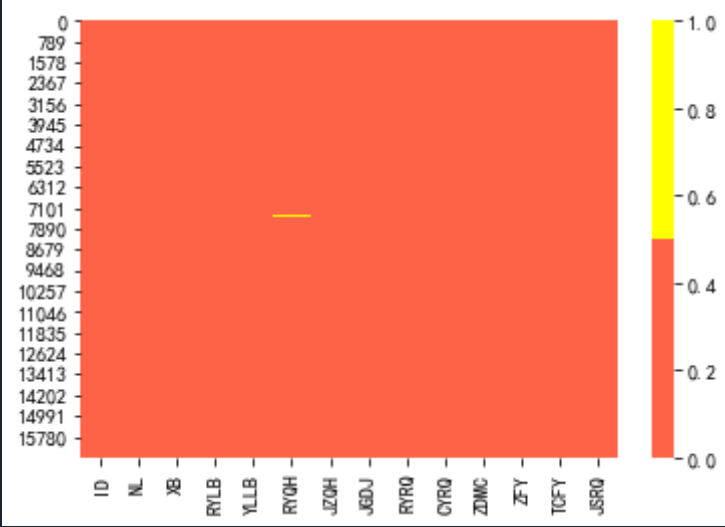
\includegraphics[scale=0.8]{figures/2.png}
\caption{数据可视化}\label{fig:label2}
\end{figure}

用热力图展现一下相关数据结构:
\begin{figure}[ht]
\centering
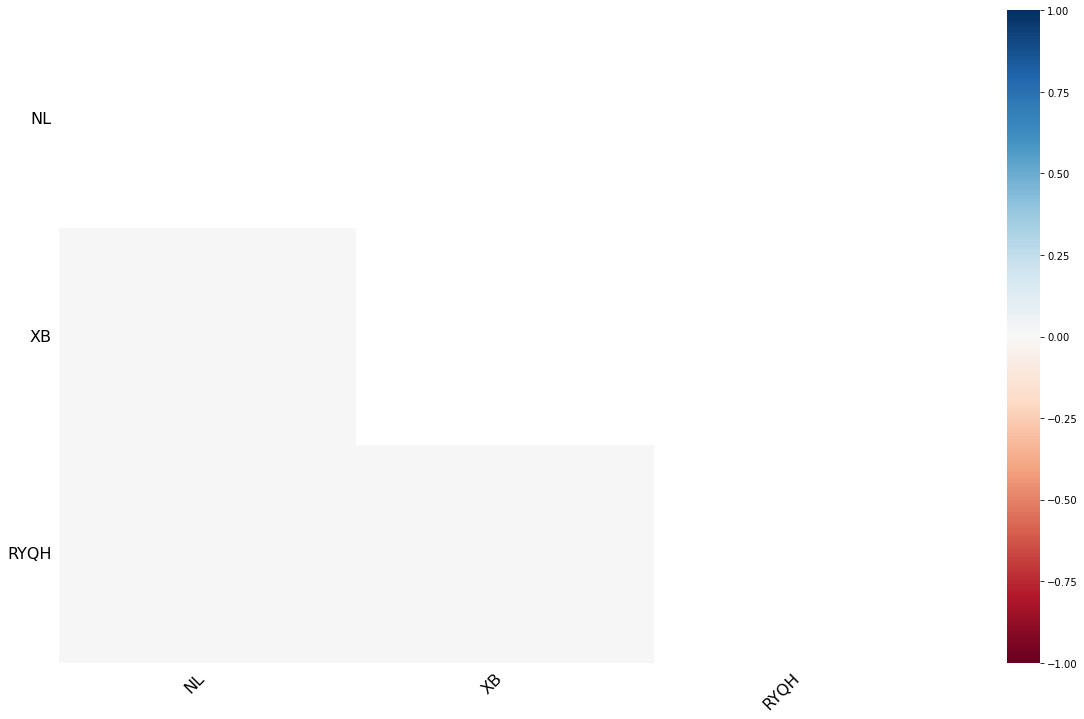
\includegraphics[scale=0.4]{figures/1.png}
\caption{数据可视化}\label{fig:label2}
\end{figure}

也可以从数据热力图看出缺失了数据

然后做数据处理,因为有年龄的缺失,所有用中位数填充,然后还一缺失的是性别,这就用众数填补:
\begin{lstlisting}
data = data.dropna(axis=0)
data.isna().sum()    # 统计缺失值
data.RYQH[data.RYQH.isnull()] = data.JZQH[data.RYQH.isnull()]
\end{lstlisting}

\section{数据可视化}

\subsection{条形图}
想用条形图方式,画出以地域的患病人数和以人们患病的地域。

以人员患病所在区域,画病例人数统计条形图

\newpage
\begin{figure}[ht]
\centering

\includegraphics[scale=0.4]{figures/3.png}
\caption{人员患病统计分配图}\label{fig:label2}
\end{figure}

以就诊区域为主,画病例人数统计图

\begin{figure}[ht]
\centering
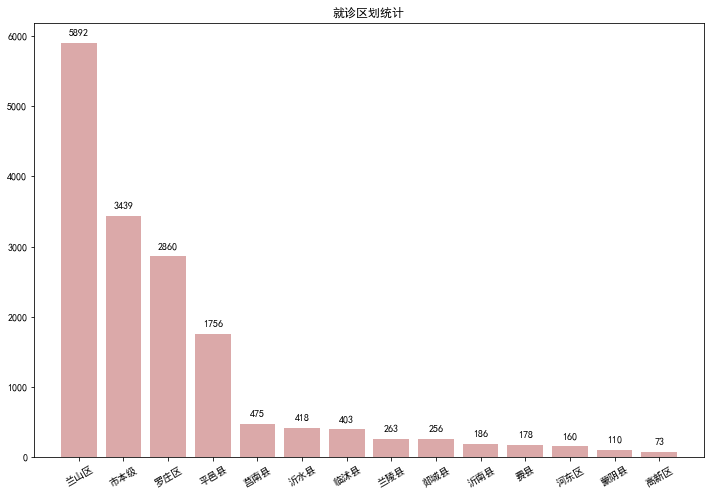
\includegraphics[scale=0.4]{figures/4.png}
\caption{按城市划分的收入分配图}\label{fig:label2}
\end{figure}

我们首先可以得出:病患的人主要集中在兰山区和罗庄区、平邑区,然后还可以得出,大家都是就近就医,没有说单单往一级医院去进行就医。所有可以得出,政府应该要平均分配,考虑这些医院的设备等问题,定时做检查,资金投入也要合理。

\subsection{相关系数热力图}
该相关系数只能度量出变量之间的线性相关关系;也就是说,相关系数越高,则变量间的线性相关程度越高。对于相关系数小的两个变量,只能说明变量间的线性相关程度弱,但不能说明变量之间不存在其它的相关关系。通过热力图,我们可以直观地看到所给数值大小的差异状况。

如下图:

\begin{figure}[ht]
\centering
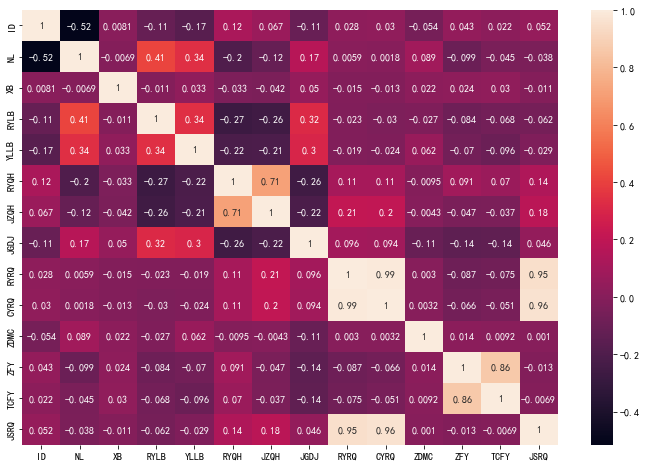
\includegraphics[scale=0.5]{figures/5.png}
\caption{数据相关系数可视化}\label{fig:label2}
\end{figure}

热力图右侧的刻度展示了不同相关系数对应的颜色深浅。从图中可以看出,权益乘数和流动负债权益比率之间的相关性较高。

\subsection{看病平均花费top10}
探究在所有病例中,为治疗此病例要花费的金额,可视化出top10,为了使政府知道那种病需要去了解用药情况,去把贵的药物价格降低,使城市居民不在害怕没钱不敢治疗。
\begin{figure}[ht]
\centering
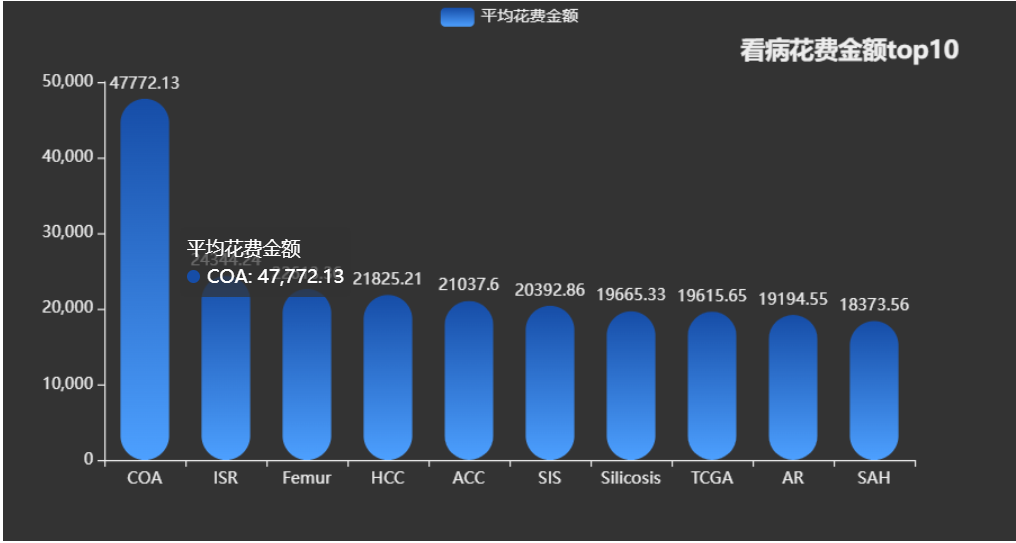
\includegraphics[scale=0.8]{figures/6.png}
\caption{看病平均花费top10}\label{fig:label2}
\end{figure}

可以看出coa也就是主动脉弓狭窄,是特别耗费钱的,比其他病都要花费多的多。

处理完数据如下表:
\begin{table}[!ht]
    \centering
    \begin{tabular}{|l|l|l|l|l|l|}
    \hline
        主动脉弓狭窄   & 动脉狭窄  &  股骨假体周围骨折 & 肝肿瘤  &  慢性丹囊炎  &  矽肺 \\ \hline
        47772.13  & 24344.24  & 22613.36  & 21825.21  & 21037.6  & 20392.86  \\ \hline
    \end{tabular}
\end{table}


\subsection{双柱状图}

因为社会舆论中存在不同医院收费不同,越是大医院收费越高问题,此次我们可视化一级医院和二级医院相同病例的平均收费情况,在理论情况下,有一定偏差,但是不存在很大偏差则可以认为医院没有越是大医院收费越高问题。证明所有医院的都是以正常标准收费。不乱收钱,可视化出结结果,让居民方向。

\begin{figure}[ht]
\centering
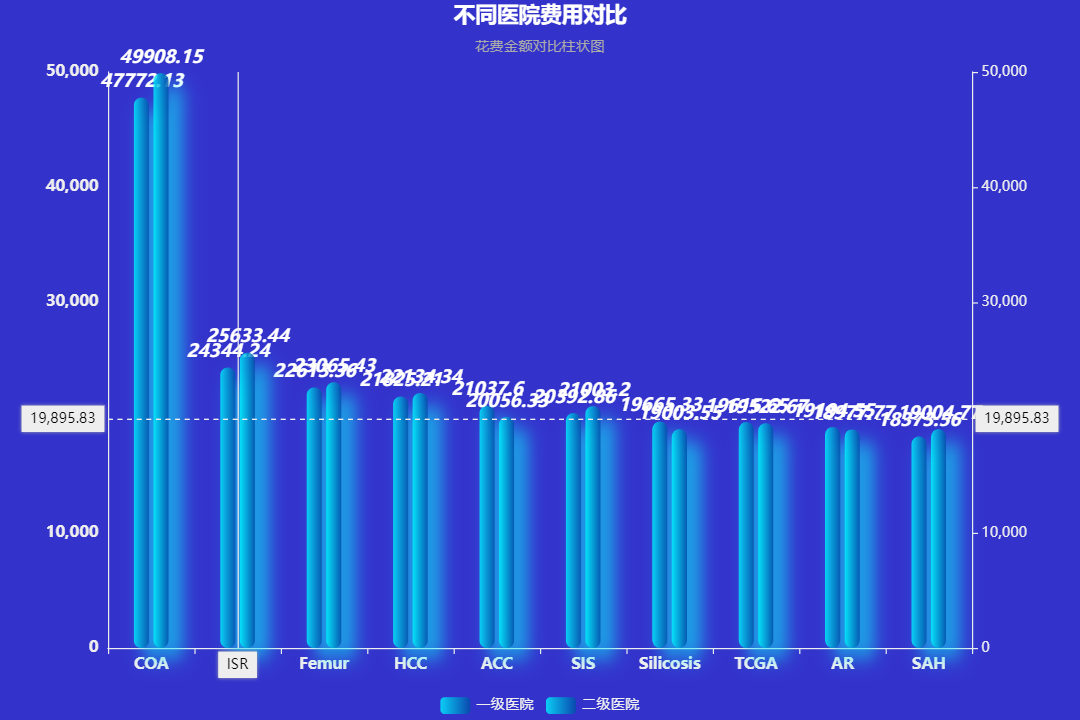
\includegraphics[scale=0.4]{figures/7.png}
\caption{医院费用对比可视化}\label{fig:label2}
\end{figure}

可以很明显看出,其实差别都不大,如果样本量足够多的情况下,误差会很小很小,所有居民不用担心医院有乱收费情况。

\subsection{饼图}
做一次调查,以所有生病人员为主题,以去过的医院为样本,画出饼图,看看是否大家都喜欢去更好的医院治病。


\begin{figure}[ht]
\centering
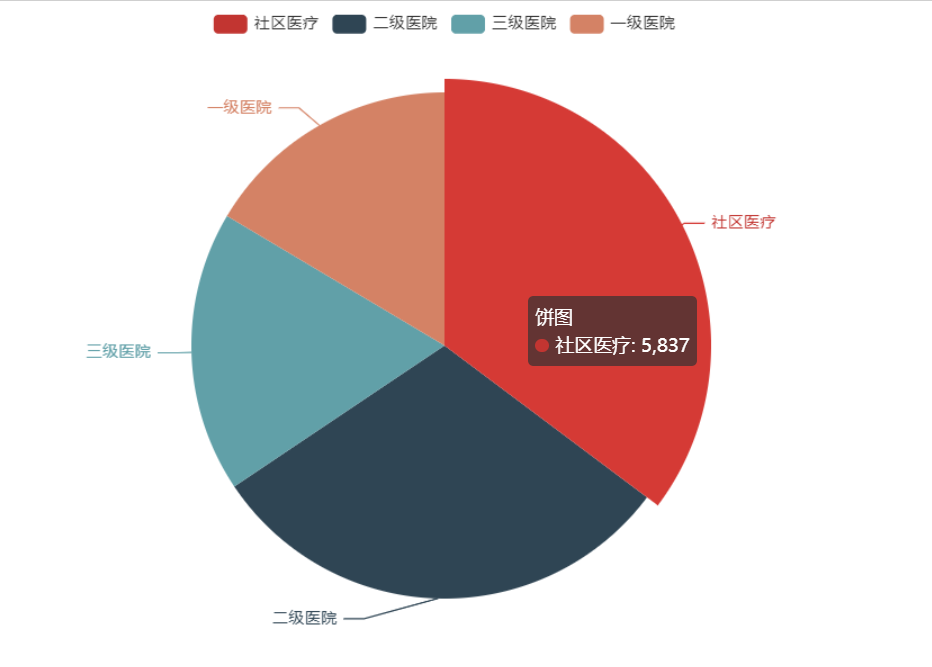
\includegraphics[scale=0.7]{figures/8.png}
\caption{各个医院接纳病人情况}\label{fig:label2}
\end{figure}

可以看出,社区医院才是最多的。说明社区医院才是居民最主要的去的医院。也可以说明居民以就近原则去治疗,并没有更喜欢去大医院治疗。

\newpage
\subsection{玫瑰图}
为了了解居民们平常最容易生什么病,生什么病最多,做一个排名,显示前20的病例排名。

\begin{figure}[ht]
\centering

\includegraphics[scale=0.7]{figures/9.png}
\caption{患病总数的排名}\label{fig:label2}
\end{figure}


可以看出,糖尿病,冠心病和高血压是主要影响居民健康的疾病。所有政府可以针对这几个疾病做出相对政策。

\newpage
\subsection{圆环图}

为了了解受病群体的工作情况,退休情况,还是离休的。画出此图表:

\begin{figure}[ht]
\centering
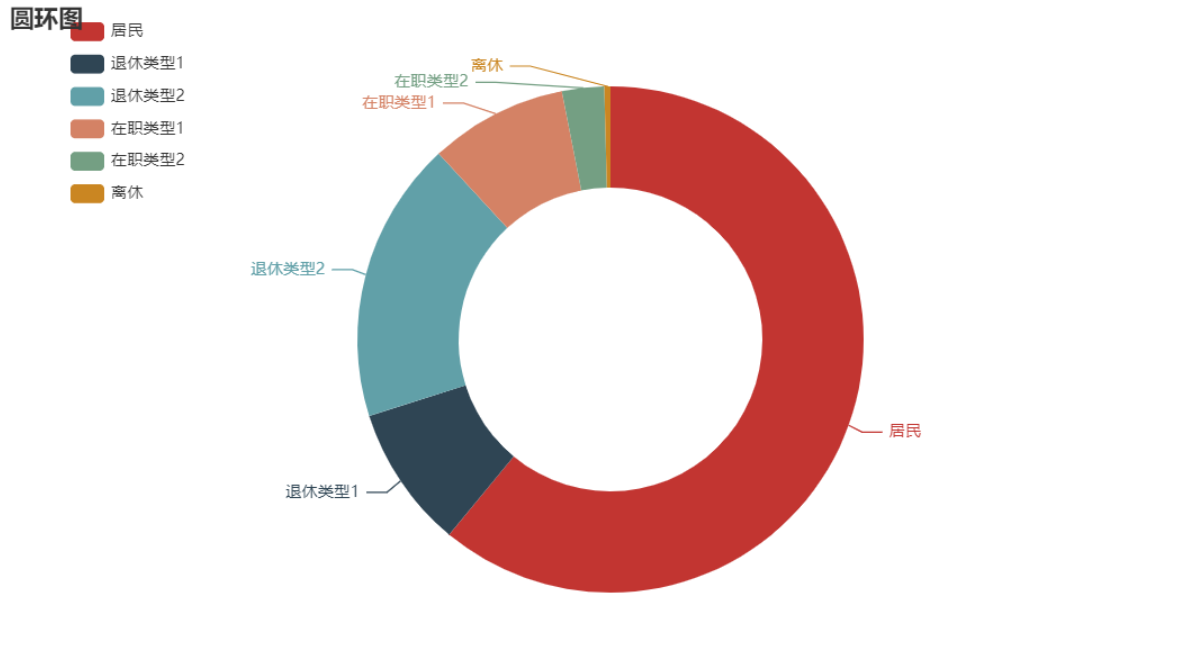
\includegraphics[scale=0.7]{figures/10.png}
\caption{各个医院病人的工作情况}\label{fig:label2}
\end{figure}

由图可得,还是居民较多,离休较少,可能也是因为生病才离休的。

\subsection{象型柱图}
查看居民,去的医院类别:

\begin{figure}[ht]
\centering

\includegraphics[scale=0.7]{figures/14.png}
\caption{去各个医院的占比}\label{fig:label2}
\end{figure}


\subsection{环形饼图}

以外环为医疗等级,内圈为性别比例做环形图。可视化如下:

\begin{figure}[ht]
\centering
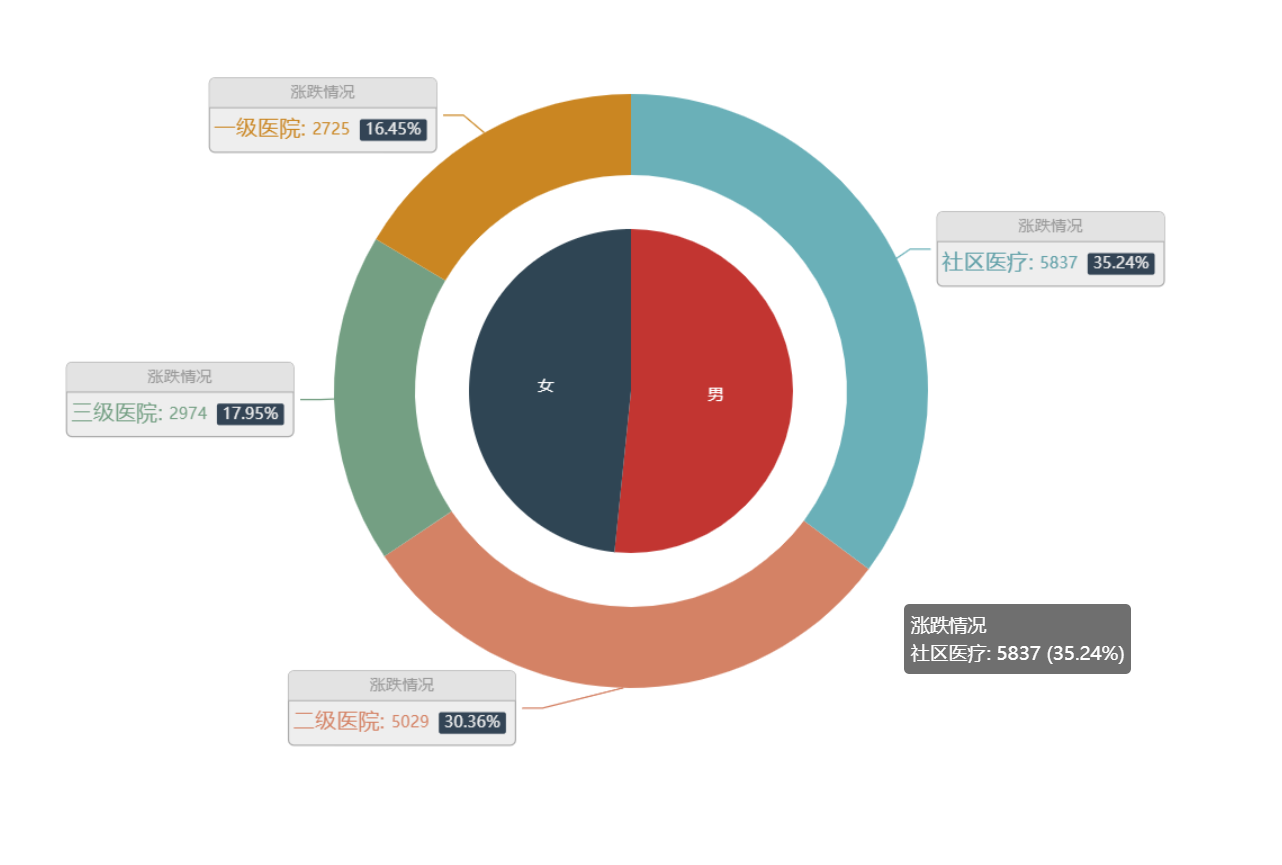
\includegraphics[scale=0.5]{figures/11.png}
\caption{医疗情况}\label{fig:label2}
\end{figure}


可以看出男女比例都很正常。而且医院收纳人的数量也是很均衡。

\subsection{以特征画图}

在所有病例中,我们以小于七岁的年龄为特征,统计出小于七岁患病的病例,画出可视化图。

\begin{figure}[ht]
\centering
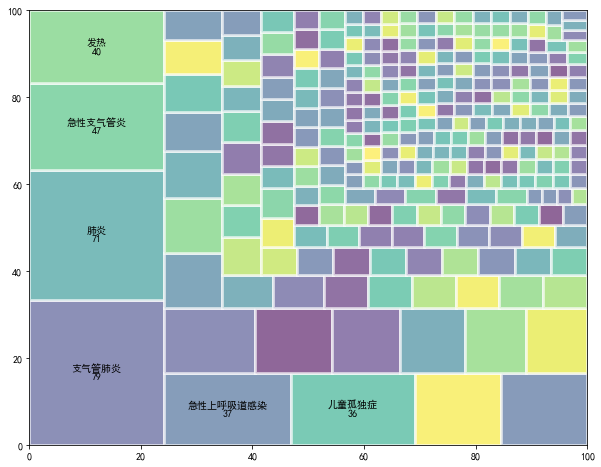
\includegraphics[scale=0.5]{figures/12.png}
\caption{儿童患病情况情况}\label{fig:label2}
\end{figure}

由此可见:支气管肺炎和肺炎比较多,其次比较少,政府主要关注儿童的肺炎疾病。并且我们可以查看,以70岁为老年所患病病例:

\begin{figure}[ht]
\centering
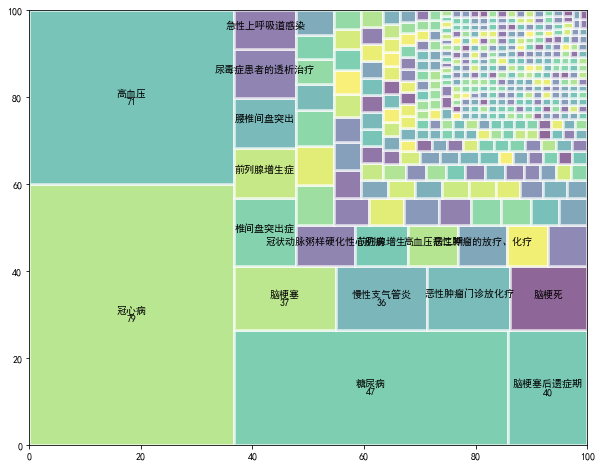
\includegraphics[scale=0.5]{figures/13.png}
\caption{老年人患病情况}\label{fig:label2}
\end{figure}

可以看出来,老年人主要是以患冠心病,高血压,糖尿病为主。

\section{数据可视化大屏}

通过汇总,我们认为做一个数据可视化大屏,可以有效地反应所有的居民就医问题与就医意愿,如图:

\begin{figure}[ht]
\centering
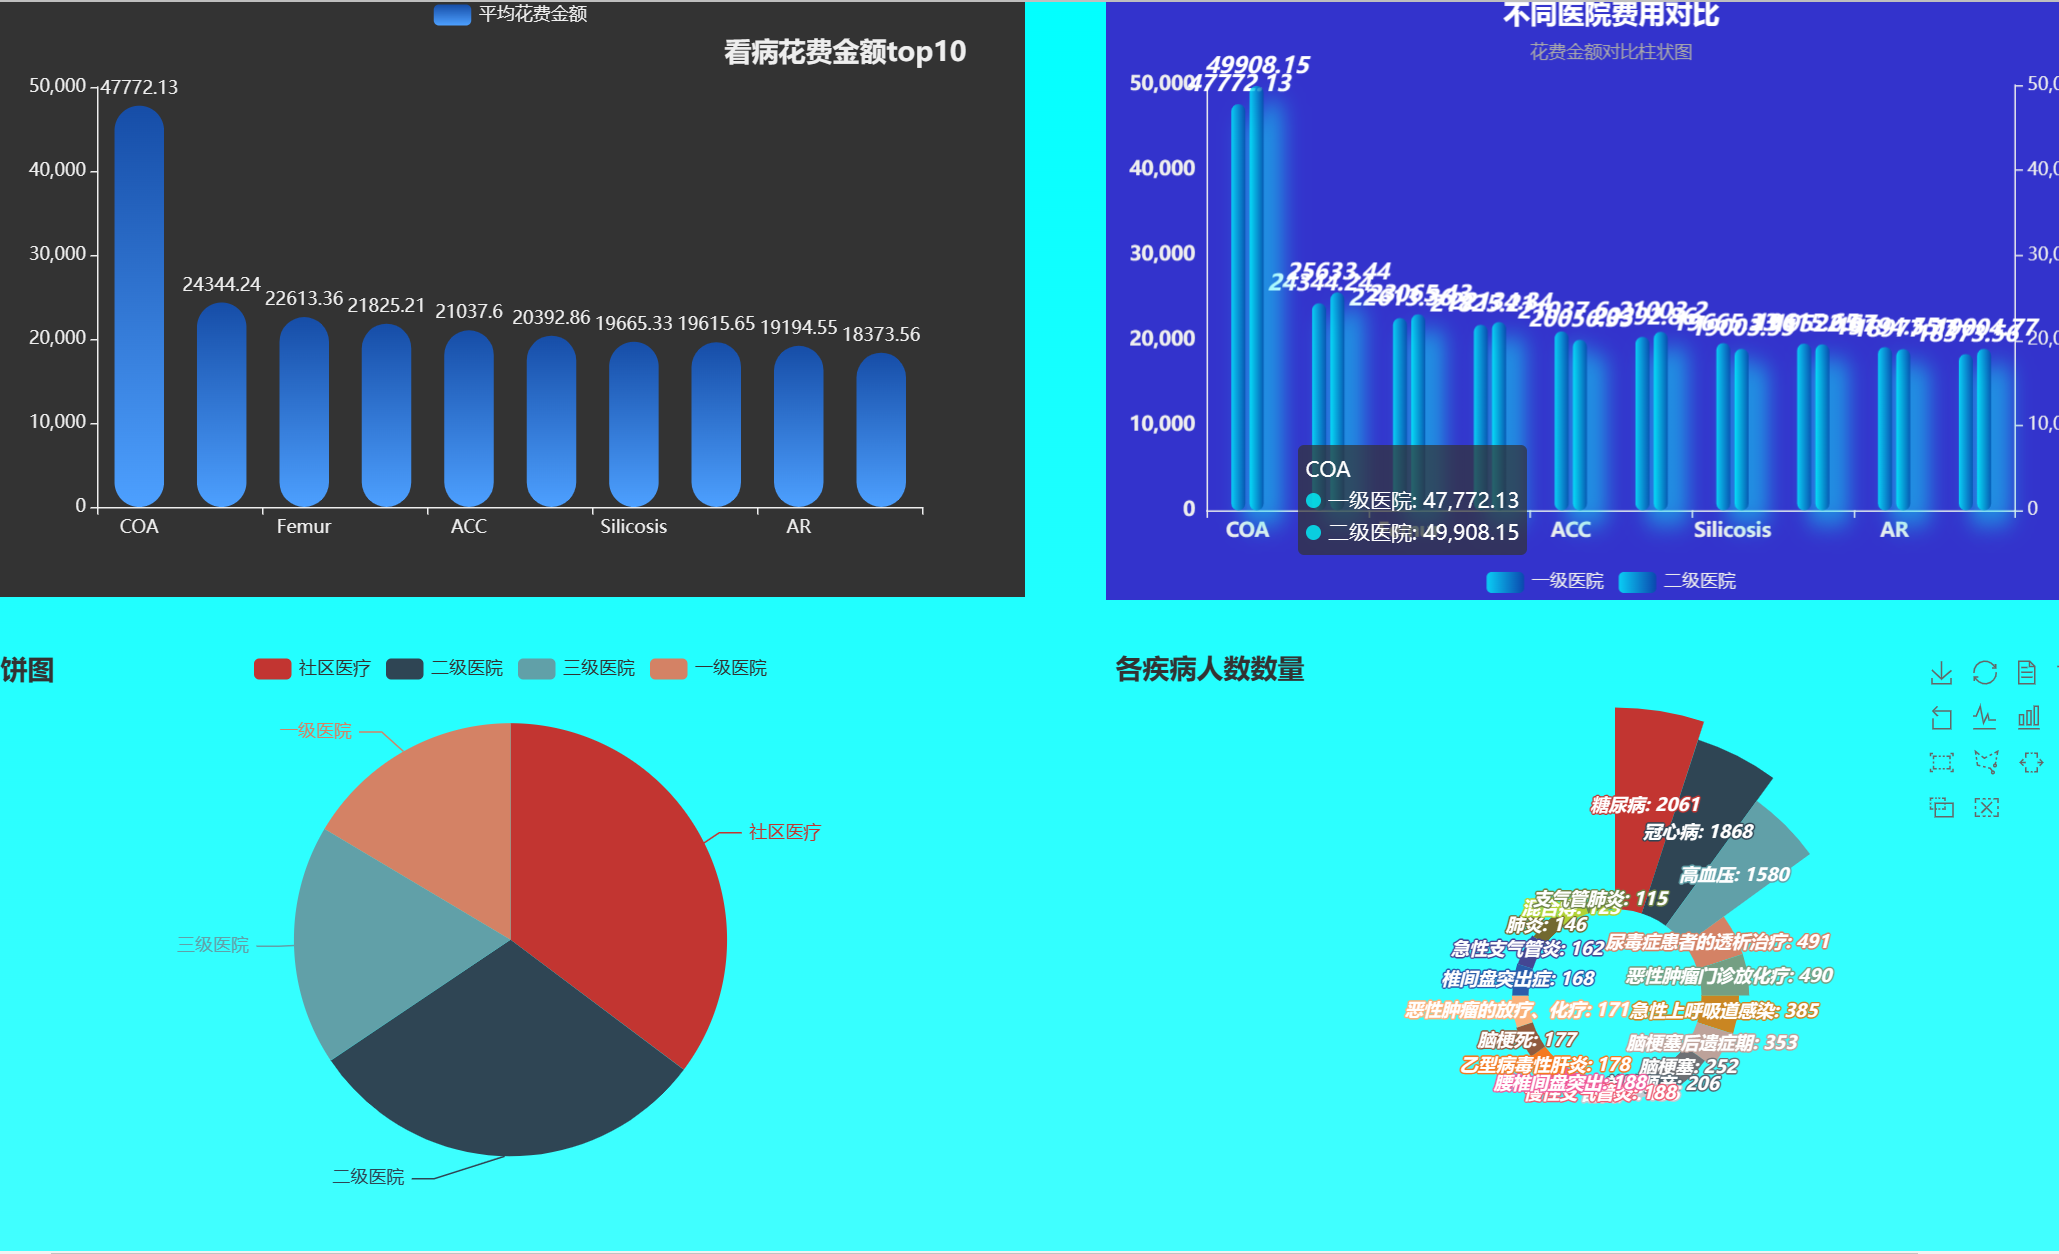
\includegraphics[scale=0.3]{figures/16.png}
\caption{可视化大屏}\label{fig:label2}
\end{figure}

\begin{figure}[ht]
\centering
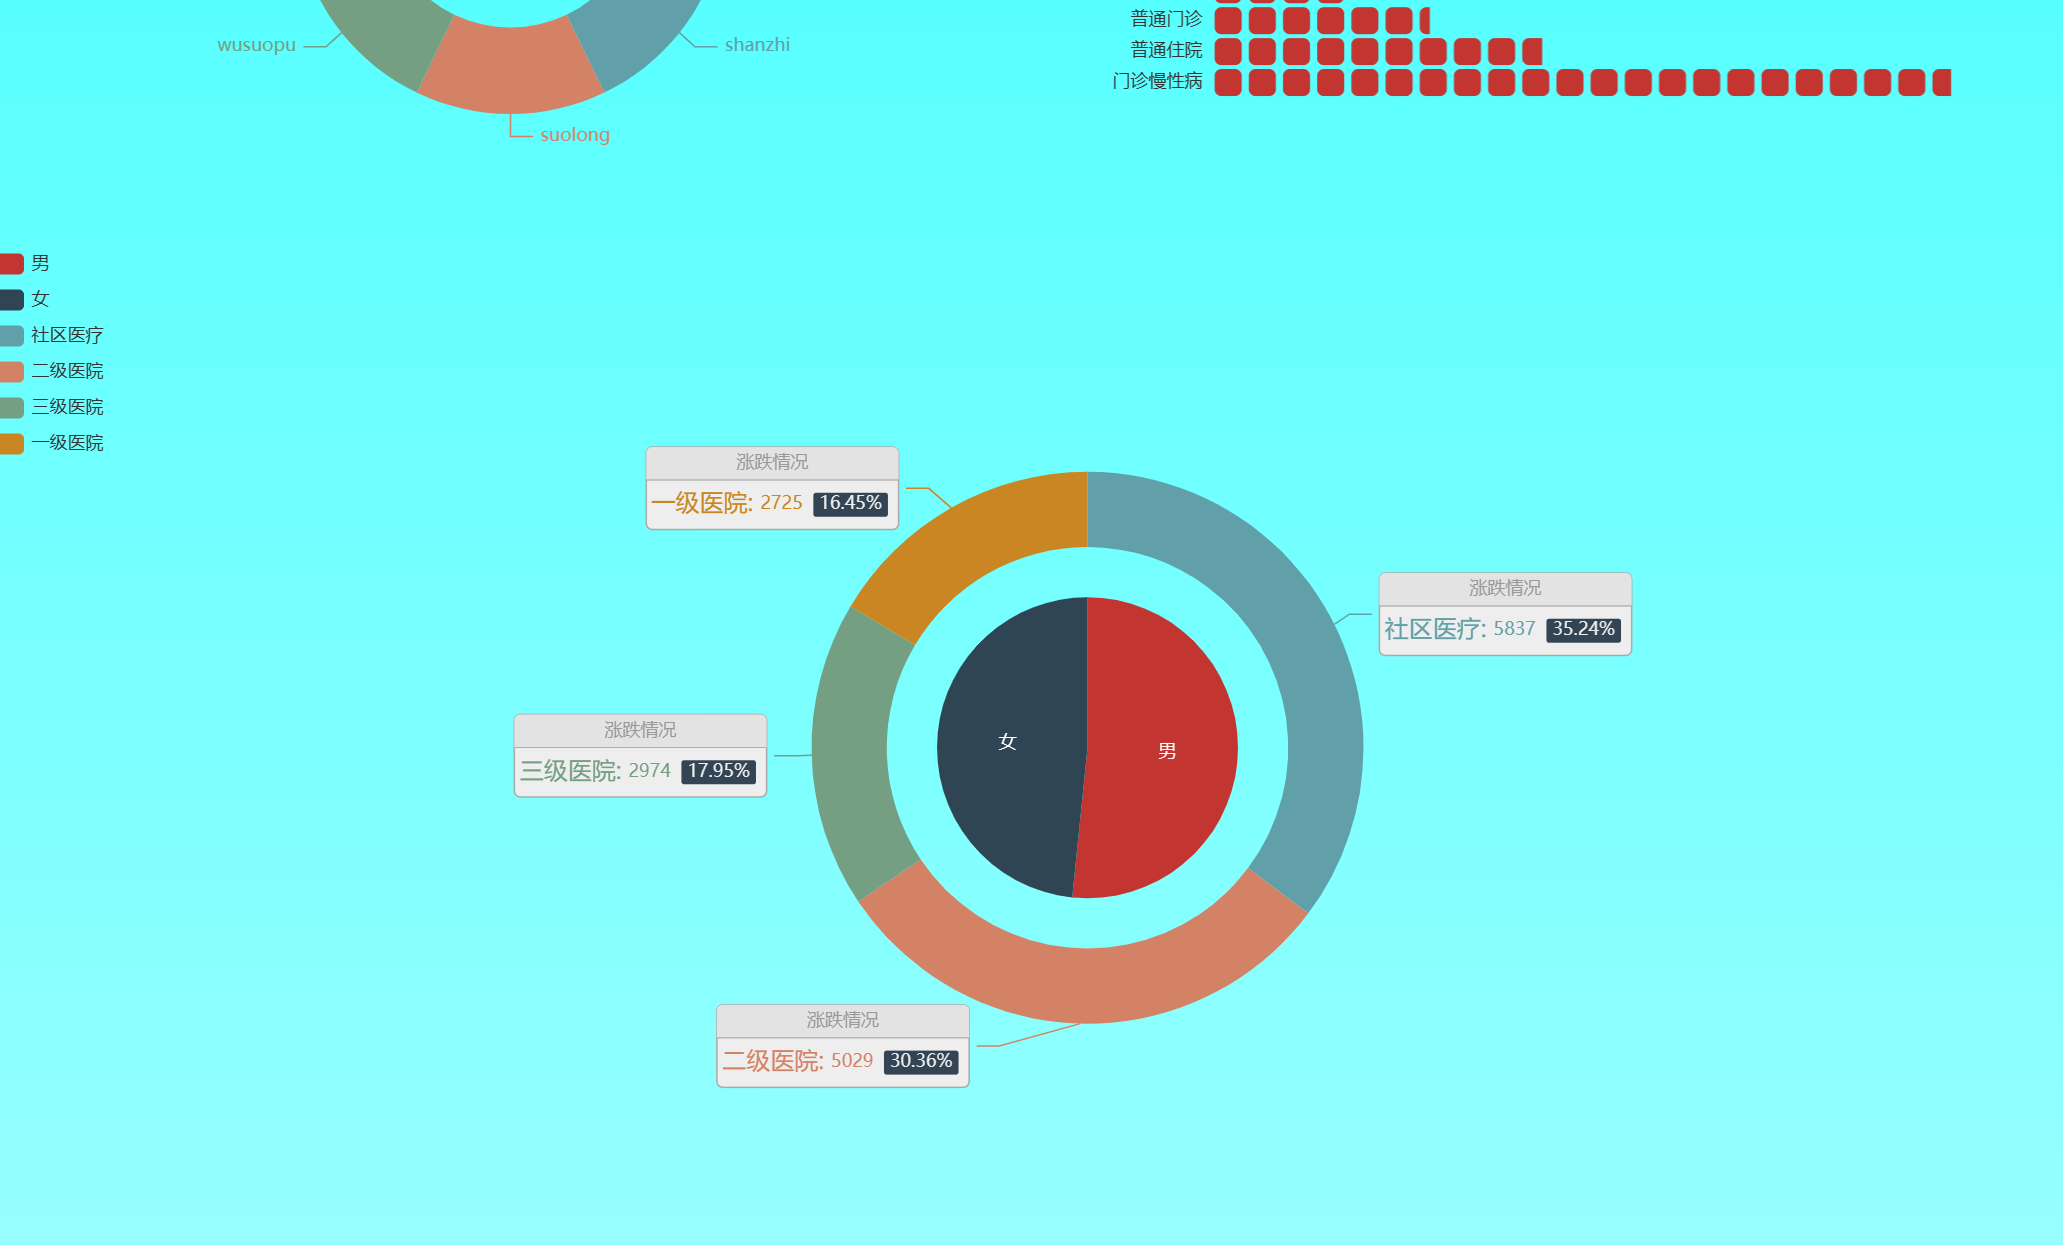
\includegraphics[scale=0.3]{figures/15.png}
\caption{可视化大屏}\label{fig:label2}
\end{figure}
\section{总结与评价}
\subsection{总结}
医疗是为了挽救生命、延长寿命、提高生存质量从而使个人效用最大化所最需要利用的、最优先利用的医疗服务或医疗措施;对于某个社会、某个群体(比如某个国家的公民)来说,医疗是指对改善全体社会公民健康、提高国民素质、推动社会发展贡献最大,最应该为全体公民所享受的医疗服务或医疗措施。

由上述分析可得,患病者花费最多的是主动脉狭窄,患病最多的是糖尿病,大部分人都是就近就医。
\subsection{评价}
优点:对数据进行数据可视化分析,沟通效率更高,与数据直接交互,能轻松理解数据。分析结果可以为当地提供一些帮助。

缺点:数据量不够大,区域不够大,数据的更新不够快,容易影响数据可视化和预测的真实性。只能针对某区域,不能应用与其他地区。



%%%%%%%%%%%%%%%%%%%%参考文献%%%%%%%%%%%%%%%%%%%%%%%%%%%%%%%%%%%%%%%%%%%%%%%%%%%%%%%%%%%%%%%%%%%%%%%%%%
\newpage

\begin{thebibliography}{99}\addcontentsline{toc}{section}{参考文献}
\wuhao{
\bibitem{huang}期刊论文.《数据可视化的基本原理与方法 (豆瓣)》.

\bibitem{jiang}期刊论文.《重症医疗数据的可视化》.

\bibitem{jiang}学习pyecharts网址.https://github.com/pyecharts/pyecharts-gallery.

\bibitem{gao}高等教育出版社. https://blog.csdn.net/weixin\_38100489/article/details/78175928

}
\end{thebibliography}

%%%%%%%%%%%%%%%%%%%%%%%%%附录%%%%%%%%%%%%%%%%%%%%%%%%%%%%%%%%%%%%%%%%%%%%%%%%%%%%%%%
\newpage


{\xiaosanhao\textbf{附\quad 录}}\addcontentsline{toc}{section}{附录}

%%%将R语言程序直接插入附录中,需要把R代码放入R文件中
%注意该R文件必须保存为UTF-8的格式
\textbf{附录1:数据可视化}
\lstinputlisting[language=python]{数据处理.py}

\textbf{附录2:数据可视化}
\begin{lstlisting}
import pandas as pd
import  numpy as np
import seaborn as sns

data = pd.read_csv(r'E:\2020paper\Data visualization\医疗数据.csv',encoding="gbk")
data.head()
data1 = {
    'ZMDC':['主动脉弓狭窄','动脉狭窄',
    '股骨假体周围骨折','肝肿瘤',
    '慢性丹囊炎','矽肺','膝关节滑膜囊肿',
    '骨恶性肿瘤','主动脉瓣关闭不全',
    '蛛网膜下腔出血'],
    'ZFY':[47772.13,24344.24,22613.36,
    21825.21,21037.6,20392.86,19665.33,
    19615.65,19194.55,18373.56]
}
df = pd.DataFrame(data1,index=['1','2','3','4','5','6','7','8','9','10'])
df.head()
df['ZMDC']
import pandas as pd
from pyecharts import options as opts
from pyecharts.charts import Bar
from pyecharts.commons.utils import JsCode
from pyecharts.faker import Faker
from pyecharts.globals import ThemeType
cc = list( df["ZMDC"].values )
cc
ccc = ['COA','ISR','Femur','HCC','ACC','SIS','Silicosis','TCGA','AR','SAH']
#画柱状图

values = []
for i in df.values:
    dic = {}
    dic["value"] = i[1]
    values.append(dic)


c = (
    Bar(init_opts=opts.InitOpts(width="750px", height="400px",theme = ThemeType.DARK ))
    .add_xaxis( ccc )
    .add_yaxis("平均花费金额", values, category_gap="40%")
    .set_series_opts(
        itemstyle_opts={
            "normal": {
                "color": JsCode(
                    """new echarts.graphic.LinearGradient(0, 0, 0, 1, [{
                offset: 0,
                color: 'rgba(22, 77, 167, 1)'
            }, {
                offset: 1,
                color: 'rgba(77, 160, 321, 1)'
            }], false)"""
                ),
                "barBorderRadius": [30, 30, 30, 30],
                "shadowColor": "rgb(77, 160, 321)",
            }
        }
    )
    .set_global_opts(title_opts=opts.TitleOpts(title="看病花费金额top10",
    pos_bottom = "87%", pos_right = "5%"))
    #.render("bar_border_radius.html")
)
c.render_notebook()
# 绘制动态榜单
month_lis = ['2019年12月','2020年1月','2020年2月']
month_data_lis = [month12_data,month1_data,month2_data]
color_function = """
        function (params) {
            if (params.value < 20000)
                return ' #FF7256';
            else if (params.value >= 20000 && params.value < 40000)
                return '#19ed95';
            else return '#3333cc';
        }
        """
# 新建一个timeline对象
t2 = Timeline(
        init_opts=opts.InitOpts(
            bg_color='#FFE4E1',  # 设置背景颜色
            theme='macarons',         # 设置主题
            width='900px',     # 设置图的宽度
            height='700px'     # 设置图的高度
        )
)
t2.add_schema(
    is_auto_play = True,    # 是否自动播放
    play_interval = 1500,   # 播放速度
    is_loop_play = True,   # 是否循环播放
)

for i,data1 in zip(month_lis,month_data_lis):
    day = i
    bar = Bar(
            init_opts=opts.InitOpts(
            bg_color='#FFE4E1',  # 设置背景颜色
            theme='essos',         # 设置主题
            width='1200px',     # 设置图的宽度
            height='600px'     # 设置图的高度
        )
    )
    bar.add_xaxis(data1['产品类别id'].tolist())
    bar.add_yaxis(
        '销售额',
        data1['销售额'].round(2).tolist(),
        category_gap="40%"
        )
    bar.reversal_axis()
    bar.set_series_opts( # 自定义图表样式
        label_opts=opts.LabelOpts(is_show=True,position = "right"), # 是否显示数据标签
        itemstyle_opts={
            "normal": {
                 "color": JsCode(color_function),       # 调整柱子颜色渐变
                'shadowBlur': 8,   # 光影大小
                "barBorderRadius": [100, 100, 100, 100],  # 调整柱子圆角弧度
                "shadowColor": "#E9B7D3", # 调整阴影颜色
                'shadowOffsetY': 6,
                'shadowOffsetX': 6,  # 偏移量
            }
        }
    )
    bar.set_global_opts(
    # 标题设置
    title_opts=opts.TitleOpts(
        title='每月各产品类别销售额top榜单', # 主标题
        subtitle='', # 副标题
        pos_left='center',  # 标题展示位置
        title_textstyle_opts=dict(color='#5A3147'), # 设置标题字体颜色
        subtitle_textstyle_opts=dict(color='#5A3147')
    ),
    legend_opts=opts.LegendOpts(
        is_show=True, # 是否显示图例
        pos_left='right', # 图例显示位置
        pos_top='3%',  #图例距离顶部的距离
        orient='vertical',  # 图例水平布局
        textstyle_opts=opts.TextStyleOpts(
            color='#5A3147',  # 颜色
            font_size='13',   # 字体大小
            font_weight='bolder',   # 加粗
    ),
    ),
    tooltip_opts=opts.TooltipOpts(
        is_show=True,  # 是否使用提示框
        trigger='axis',  # 触发类型
        is_show_content = True,
        trigger_on='mousemove|click',  # 触发条件,点击或者悬停均可出发
        axis_pointer_type='cross',  # 指示器类型,鼠标移动到图表区可以查看效果
        # formatter = '{a}<br>{b}:{c}人'  # 文本内容
    ),
    yaxis_opts=opts.AxisOpts(
        is_show=True,
        splitline_opts=opts.SplitLineOpts(is_show=False), # 分割线
        axistick_opts=opts.AxisTickOpts(is_show=False), # 刻度不显示
        axislabel_opts=opts.LabelOpts(  # 坐标轴标签配置
            font_size=13,  # 字体大小
            font_weight='bolder' # 字重
        ),
    ),   # 关闭Y轴显示
    xaxis_opts=opts.AxisOpts(
        boundary_gap=True,    # 两边不显示间隔
        axistick_opts=opts.AxisTickOpts(is_show=True),  # 刻度不显示
        splitline_opts=opts.SplitLineOpts(is_show=False),  # 分割线不显示
        axisline_opts=opts.AxisLineOpts(is_show=True),  # 轴不显示
        axislabel_opts=opts.LabelOpts(  # 坐标轴标签配置
            font_size=13,  # 字体大小
            font_weight='bolder' # 字重
            ),
        ),
    )

    t2.add(bar, day)

t2.render_notebook()
pro_category = {
    'ZMDC':['COA','ISR','Femur','HCC','ACC','SIS','Silicosis','TCGA','AR','SAH'],
    #'ZMDC':['主动脉弓狭窄','动脉狭窄','股骨假体周围骨折','肝肿瘤','慢性丹囊炎',
    '矽肺','膝关节滑膜囊肿','骨恶性肿瘤','主动脉瓣关闭不全','蛛网膜下腔出血'],
    '一级医院':[47772.13,24344.24,22613.36,21825.21,
    21037.6,20392.86,19665.33,19615.65,19194.55,18373.56],
    '二级医院':[49908.15,25633.44,23065.43,22134.34,
    20056.33,21003.2,19003.55,19522.67,18977.77,19004.77],
}
pro_category = pd.DataFrame(pro_category,index=['1','2',
'3','4','5','6','7','8','9','10'])
pro_category

def echarts_bar(x,y,y2,title = '主标题'
,subtitle = '副标题',label = '图例',label2 = '图例2',color='color'):
    """
    x: 函数传入x轴标签数据
    y:函数传入y轴数据
    title:主标题
    subtitle:副标题
    label:图例
    """
    bar = Bar(
            init_opts=opts.InitOpts(
            bg_color='#3333cc',  # 设置背景颜色
            theme='dark',         # 设置主题
            width='900px',     # 设置图的宽度
            height='600px'     # 设置图的高度
        )
    )
    bar.add_xaxis(x)
    bar.add_yaxis(label,y,
        label_opts=opts.LabelOpts(is_show=True) # 是否显示数据
        ,category_gap="60%" # 柱子宽度设置
        ,yaxis_index=0
        )
    bar.add_yaxis(label2,y2,
        label_opts=opts.LabelOpts(is_show=True) # 是否显示数据
        ,category_gap="60%" # 柱子宽度设置
        ,yaxis_index=1
    )
    bar.set_series_opts( # 自定义图表样式
        label_opts=opts.LabelOpts(
            is_show=True,
            position='top', # position 标签的位置 可选 'top','left',
            'right','bottom','inside','insideLeft','insideRight'
            font_size=15,
            color= 'white',
            font_weight = 'bolder',  # font_weight 文字字体的粗细
             'normal','bold','bolder','lighter'
            font_style = 'oblique',  # font_style 文字字体的风格,
            可选 'normal','italic','oblique'
            ),
        itemstyle_opts={
            "normal": {
                "color": color,       # 调整柱子颜色渐变
                'shadowBlur': 15,   # 光影大小
                "barBorderRadius": [100, 100, 100, 100],  # 调整柱子圆角弧度
                "shadowColor": "#0EEEF9", # 调整阴影颜色
                'shadowOffsetY': 10,
                'shadowOffsetX': 10,  # 偏移量
            }
        }
    )
    bar.set_global_opts(
        # 标题设置
        title_opts=opts.TitleOpts(
            title=title, # 主标题
            subtitle=subtitle, # 副标题
            pos_left='center',  # 标题展示位置
            title_textstyle_opts=dict(color='#fff') # 设置标题字体颜色
        ),
        # 图例设置
        legend_opts=opts.LegendOpts(
            is_show=True, # 是否显示图例
            pos_bottom='bottom',
            orient='horizontal'  # 图例水平布局
        ),
        tooltip_opts=opts.TooltipOpts(
            is_show=True,  # 是否使用提示框
            trigger='axis',  # 触发类型
            is_show_content = True,
            trigger_on='mousemove|click',  # 触发条件,点击或者悬停均可出发
            axis_pointer_type='cross',  # 指示器类型,鼠标移动到图表区可以查看效果
        ),
        yaxis_opts=opts.AxisOpts(
            is_show=True,
            splitline_opts=opts.SplitLineOpts(is_show=False), # 分割线
            axistick_opts=opts.AxisTickOpts(is_show=False), # 刻度不显示
            axislabel_opts=opts.LabelOpts(  # 坐标轴标签配置
                font_size=13,  # 字体大小
                font_weight='bolder' # 字重
            ),
        ),   # 关闭Y轴显示
        xaxis_opts=opts.AxisOpts(
            boundary_gap=True,    # 两边不显示间隔
            axistick_opts=opts.AxisTickOpts(is_show=True),  # 刻度不显示
            splitline_opts=opts.SplitLineOpts(is_show=False),  # 分割线不显示
            axisline_opts=opts.AxisLineOpts(is_show=True),  # 轴不显示
            axislabel_opts=opts.LabelOpts(  # 坐标轴标签配置
                font_size=13,  # 字体大小
                font_weight='bolder' # 字重
            ),
        ),
    )
    bar.extend_axis(yaxis=opts.AxisOpts())
    return bar.render_notebook()

color = {
       'type': 'linear',
        'x': 0,
        'y': 0,
        'y2': 0,
        'x2': 1,
        'colorStops': [
            {'offset': 0, 'color': 'rgba(0, 244, 255, 0.8)' },
            {'offset': 1, 'color': 'rgba(0, 77, 167, 0.8)'}],
        'global': False
    }
echarts_bar(pro_category['ZMDC'].tolist(), pro_category['一级医院'].tolist(),
            pro_category['二级医院'].tolist(), title='不同医院费用对比', subtitle='花费金额对比柱状图',
            label='一级医院', label2='二级医院', color=color)

shuju = data['JGDJ'].value_counts()
shuju

from pyecharts.charts import *
from pyecharts import options as opts
'''饼图'''
L1 = ["社区医疗","二级医院","三级医院","一级医院"]
num = [5837,5029,2974,2725]
C = Pie()
C.add("饼图",[list(z) for z in zip(L1,num)])
C.set_global_opts(title_opts=opts.TitleOpts(title="饼图"))
#C.set_series_opts(label_opts=opts.TitleOpts(formatter="{b}:{c}"))
C.render_notebook()

from pyecharts import options as opts
from pyecharts.charts import Pie
from pyecharts.commons.utils import JsCode
from pyecharts.globals import ThemeType

df1 = data['ZDMC'].value_counts()
df0  = df1.head(20)

# color={
#        'type': 'linear',
#         'x': 0,
#         'y': 1,
#         'x2': 0,
#         'y2': 0,
#         'colorStops': [
#             {'offset': 0, 'color': 'black' },
#             {'offset': 1, 'color': 'orange'}],
#         'global': False
#     }
c1 = (
    Pie()
    .add('test', [list(z) for z in zip(df0.index.values.tolist(), df0.values.tolist())],
         radius=['30%', '100%'],
         center=['50%', '60%'],
         rosetype='area',
         )
    .set_global_opts(title_opts=opts.TitleOpts(title='地区景点数量'),
                     legend_opts=opts.LegendOpts(is_show=False),
                     toolbox_opts=opts.ToolboxOpts()
                    )
    .set_series_opts(label_opts=opts.LabelOpts(is_show=True, position='inside', font_size=12,
                                               formatter='{b}: {c}', font_style='italic',
                                               font_weight='bold', font_family='Microsoft YaHei'
                                               ),
#                     itemstyle_opts=opts.ItemStyleOpts(color=color)
                    )
)
c1.render_notebook()

dff = data['RYLB'].value_counts()
dff

from pyecharts.charts import *
from pyecharts import options as opts
'''圆环图'''
L1 = ["居民","退休类型1","退休类型2","在职类型1","在职类型2","离休"]
num = [10104,1510,2984,1458,445,64]
C = Pie()
'''radius调节大小'''
C.add("圆环图",[list(z) for z in zip(L1,num)],radius=["45%","75%"])
C.set_global_opts(title_opts=opts.TitleOpts(title="圆环图"),
legend_opts=opts.LegendOpts(orient="vertical",pos_top="2%",pos_left="5%"))
C.render_notebook()

dfff = data['XB'].value_counts()
dfff

import pyecharts.options as opts
from pyecharts.charts import Pie

"""

"""

inner_x_data = ["男", "女"]
inner_y_data = [8551 , 8012]
inner_data_pair = [list(z) for z in zip(inner_x_data, inner_y_data)]

outer_x_data = ["社区医疗","二级医院","三级医院","一级医院"]
outer_y_data = [5837,5029,2974,2725]
outer_data_pair = [list(z) for z in zip(outer_x_data, outer_y_data)]

c = (
    Pie(init_opts=opts.InitOpts(width="1600px", height="800px"))
    .add(
        series_name="涨跌情况",
        data_pair=inner_data_pair,
        radius=[0, "30%"],
        label_opts=opts.LabelOpts(position="inner"),
    )
    .add(
        series_name="涨跌情况",
        radius=["40%", "55%"],
        data_pair=outer_data_pair,
        label_opts=opts.LabelOpts(
            position="outside",
            formatter="{a|{a}}{abg|}\n{hr|}\n {b|{b}: }{c}  {per|{d}%}  ",
            background_color="#eee",
            border_color="#aaa",
            border_width=1,
            border_radius=4,
            rich={
                "a": {"color": "#999", "lineHeight": 22, "align": "center"},
                "abg": {
                    "backgroundColor": "#e3e3e3",
                    "width": "100%",
                    "align": "right",
                    "height": 22,
                    "borderRadius": [4, 4, 0, 0],
                },
                "hr": {
                    "borderColor": "#aaa",
                    "width": "100%",
                    "borderWidth": 0.5,
                    "height": 0,
                },
                "b": {"fontSize": 16, "lineHeight": 33},
                "per": {
                    "color": "#eee",
                    "backgroundColor": "#334455",
                    "padding": [2, 4],
                    "borderRadius": 2,
                },
            },
        ),
    )
    .set_global_opts(legend_opts=opts.LegendOpts(pos_left="left", orient="vertical"))
    .set_series_opts(
        tooltip_opts=opts.TooltipOpts(
            trigger="item", formatter="{a} <br/>{b}: {c} ({d}%)"
        )
    )
    .render_notebook()
)

c

dffff = data['YLLB'].value_counts()
dffff

from pyecharts import options as opts
from pyecharts.charts import PictorialBar
from pyecharts.globals import SymbolType

location = ['门诊慢性病' ,'普通住院' , '普通门诊',' 转省外住院特殊疾病门诊 ', '转省内住院无责任人意外伤害' ,'生育住院'    ,
            '转省外门诊慢性病' ,'转省内门诊慢性病'  ,'大病购药' ,'机关事业单位生育住院' ,'住院前急诊' ,'转省平台住院','单病种住院']
values = [7245, 3222 ,2117, 1334 ,1023, 490 , 423 ,387 ,194, 68 ,36,  13 , 10 , 2,1]

c = (
    PictorialBar()
    .add_xaxis(location)
    .add_yaxis(
        "",
        values,
        label_opts=opts.LabelOpts(is_show=False),
        symbol_size=18,
        symbol_repeat="fixed",
        symbol_offset=[0, 0],
        is_symbol_clip=True,
        symbol=SymbolType.ROUND_RECT,
    )
    .reversal_axis()
    .set_global_opts(
        title_opts=opts.TitleOpts(title="医疗类别"),
        xaxis_opts=opts.AxisOpts(is_show=False),
        yaxis_opts=opts.AxisOpts(
            axistick_opts=opts.AxisTickOpts(is_show=False),
            axisline_opts=opts.AxisLineOpts(
                linestyle_opts=opts.LineStyleOpts(opacity=0)
            ),
        ),
    )
    .render_notebook()
    #.render("pictorialbar_base.html")
)
c

\end{lstlisting}



\end{document}
